%\modeCorrection

%%%% début de la page
\renewcommand{\thesection}{\textcolor{red}{Partie \Roman{section} -}}
\renewcommand{\thesubsection}{\textcolor{red}{\Roman{section}.\arabic{subsection}}}
\renewcommand{\thesubsubsection}{\textcolor{red}{\Roman{section}.\arabic{subsection}.\alph{subsubsection}}}

\setcounter{section}{0}
\setcounter{document}{0}
\enTeteTP{12}{\'{E}tudes des composés ioniques}

\begin{center}
\begin{mdframed}[style=titr, leftmargin=60pt, rightmargin=60pt, innertopmargin=7pt, innerbottommargin=7pt, innerrightmargin=8pt, innerleftmargin=8pt]

\begin{center}
\large{\textbf{TP 12 : \'{E}tude des composés ioniques
}}
\end{center}
\end{mdframed}
\end{center}


%%%% objectifs
\begin{tcolorbox}[colback=blue!5!white,colframe=blue!75!black,title=Objectifs de la séance :]
\begin{itemize}
    \item Proposer et réaliser un protocole expérimental pour identifier des ions en solution  ;
    \item Exploiter l’électroneutralité de la matière pour associer des espèces ioniques et déterminer la formule d’un composé ionique ;
\end{itemize}
\end{tcolorbox}

%%%% Consignes
\begin{tcolorbox}[colback=red!5!white,colframe=red!75!black,title= Consignes :]
\begin{itemize}
    \item Faire attention au matériel lors de son utilisation ;
\end{itemize}
\end{tcolorbox}

%%%% contexte

\begin{tcolorbox}[colback=orange!5!white,colframe=orange!75!black,title= Contexte : à quoi sert le nigari ? :]

\begin{minipage}{0.75\textwidth}
    Vous avez retrouvé dans votre cuisine un pot de nigari, un solide ionique naturel commercialisé sous forme de paillettes. Vous vous rappelez que ce nigari vous avez été recommandé pour les effets positifs qu'il pourrait avoir sur votre corps. Malheureusement, une partie de l’étiquette du pot de nigari s’est effacée et vous ne savez plus exactement pourquoi il vous avait été recommandé. 
\end{minipage}
\begin{minipage}{0.2\textwidth}
\begin{center}
    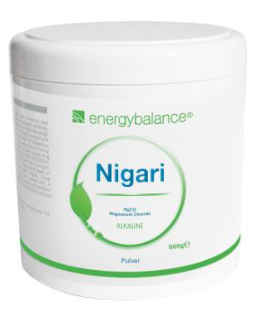
\includegraphics[scale=0.7]{Images/Nigari.PNG}
\end{center}
    
\end{minipage}
\\
\problematique{Commment retrouver les bienfaits du nigari pour la santé ?}
\end{tcolorbox}


\begin{mdframed}[style=autreexo]
\textbf{\bsc{Liste du matériel}}
\vspace{-0.5cm}
\begin{multicols}{2}
\begin{itemize}
    \item Des paillettes de nigari ;
    \item Une solution d'oxalate d'ammonium ;
    \item Une solution d'hydroxyde de sodium ;
    \item Une solution de nitrate d'argent ;
    \item Une pissette d'eau distillée ; 
    \item Une spatule ;
    \item Des tubes à essais ;
    \item Des béchers ;
\end{itemize}
\end{multicols}
\end{mdframed}

\begin{doc}{Pictogrammes de sécurité}
    \begin{tabular}{|c|c|C{0.25}|c|}
    \hline
     Solutions  & Oxalate d'ammonium & Hydroxyde de sodium (soude) & Nitrate d'argent \\ \hline
         Pictogramme & 
\includegraphics[scale=0.10]{Images/SGH07_PointExclamation.jpg} & 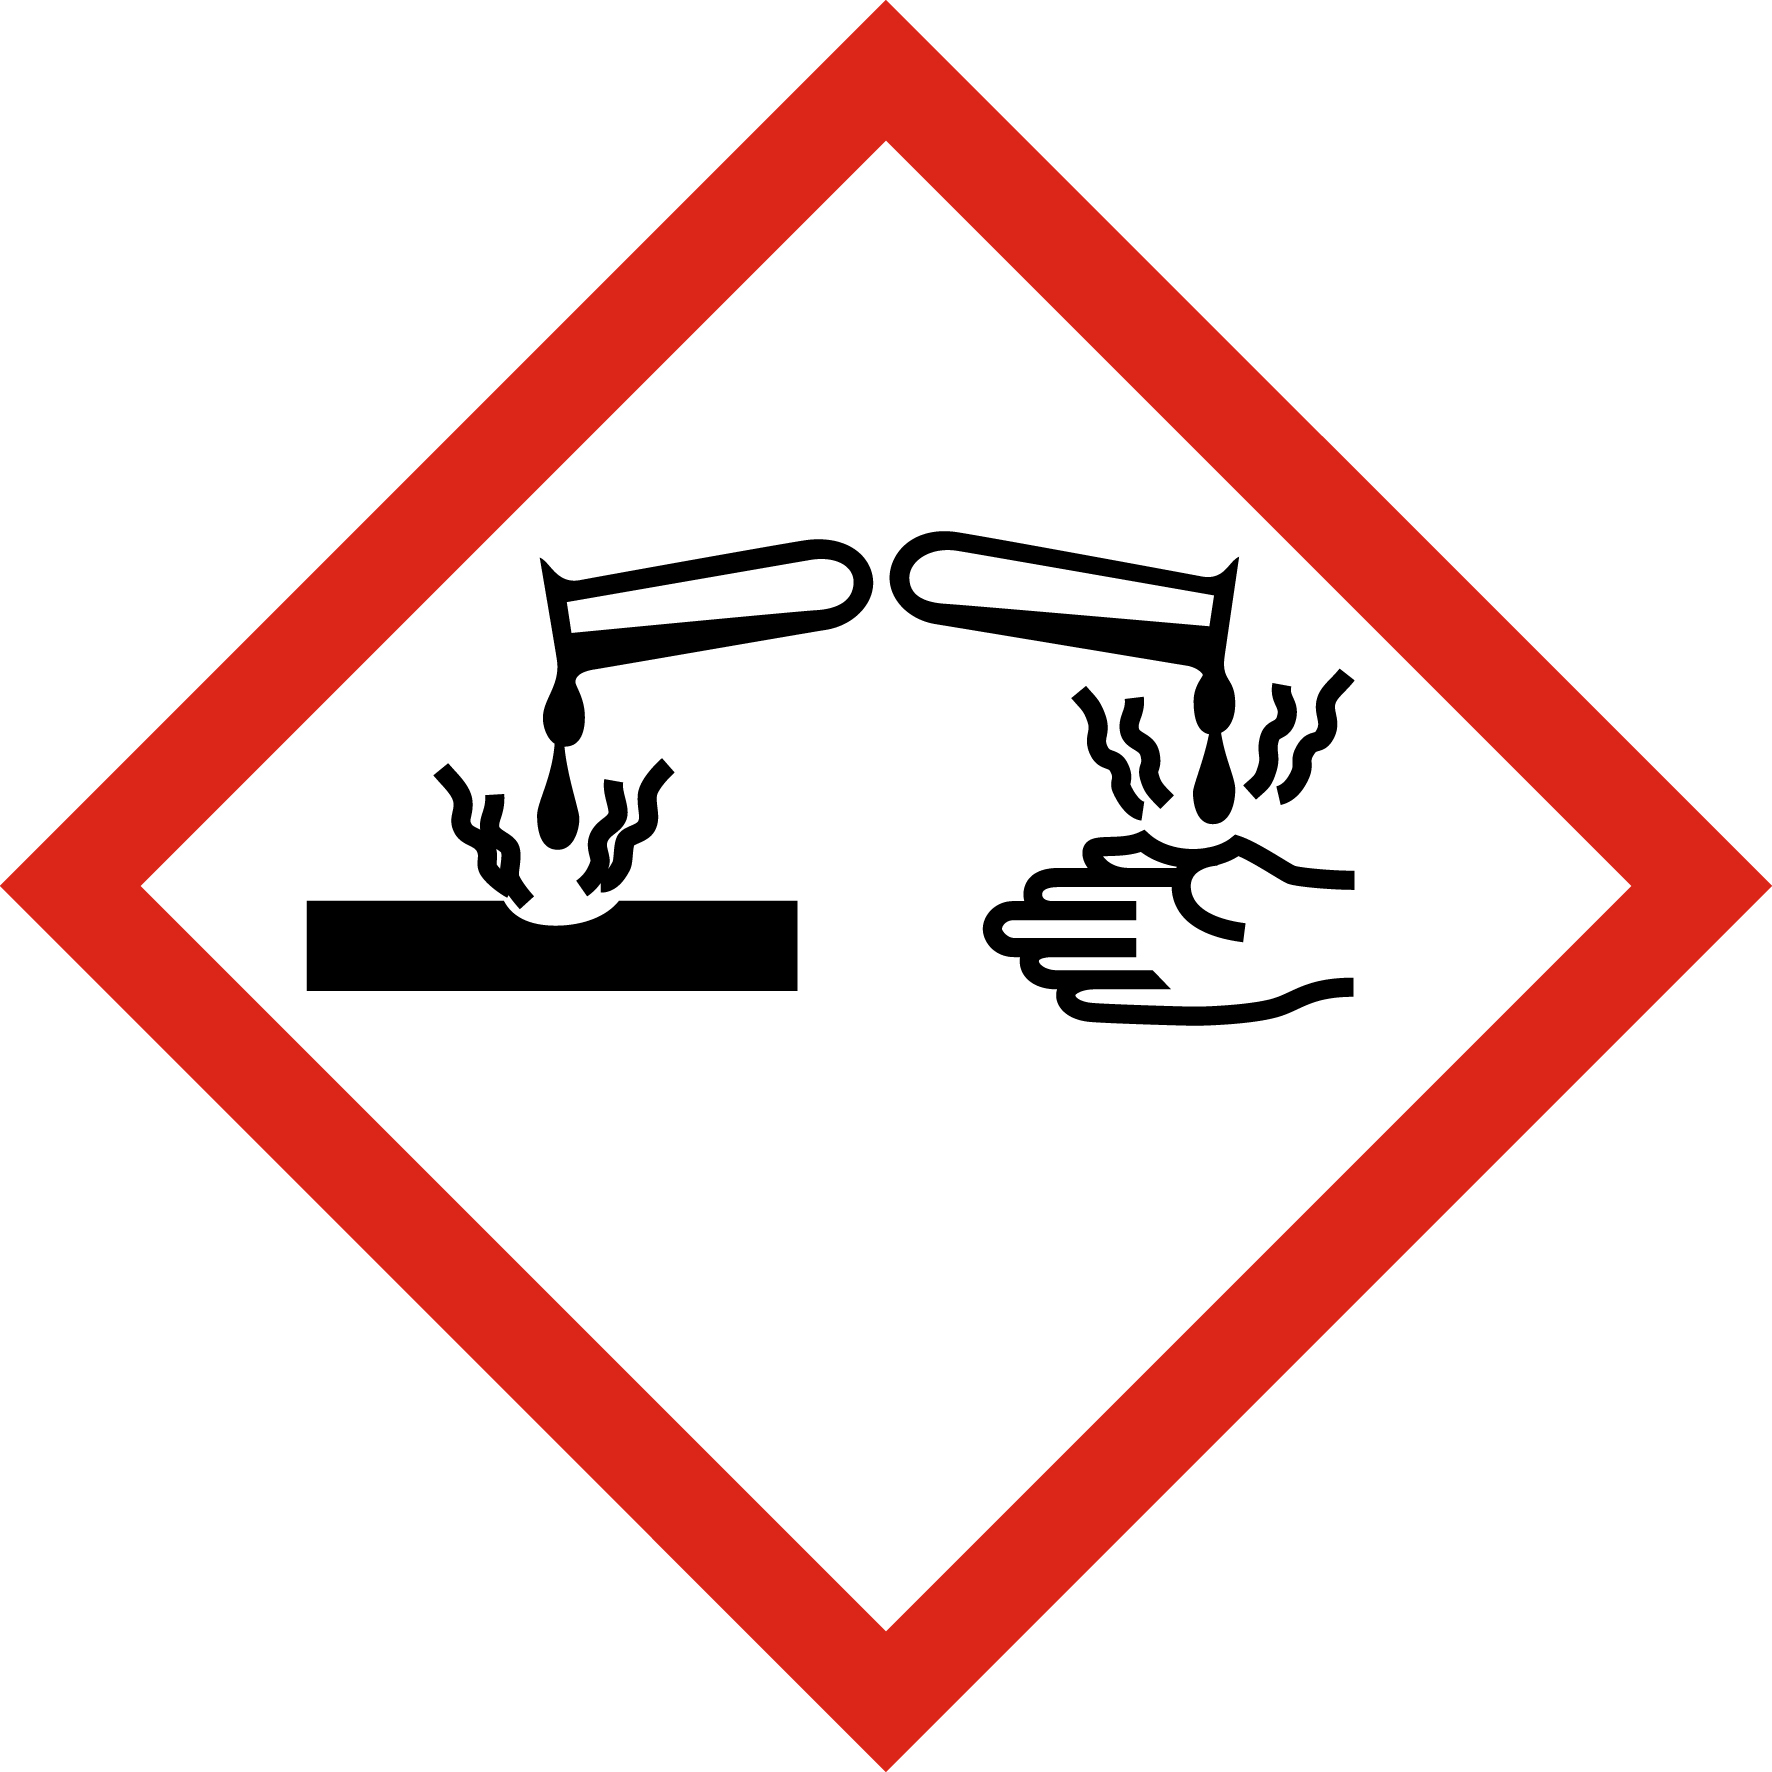
\includegraphics[scale=0.10]{Images/SGH05_Corrosion.jpg} & 
\includegraphics[scale=0.1]{Images/SGH09_Environnement.jpg} 
\includegraphics[scale=0.1]{Images/SGH03_FlammeSurCercle.jpg} 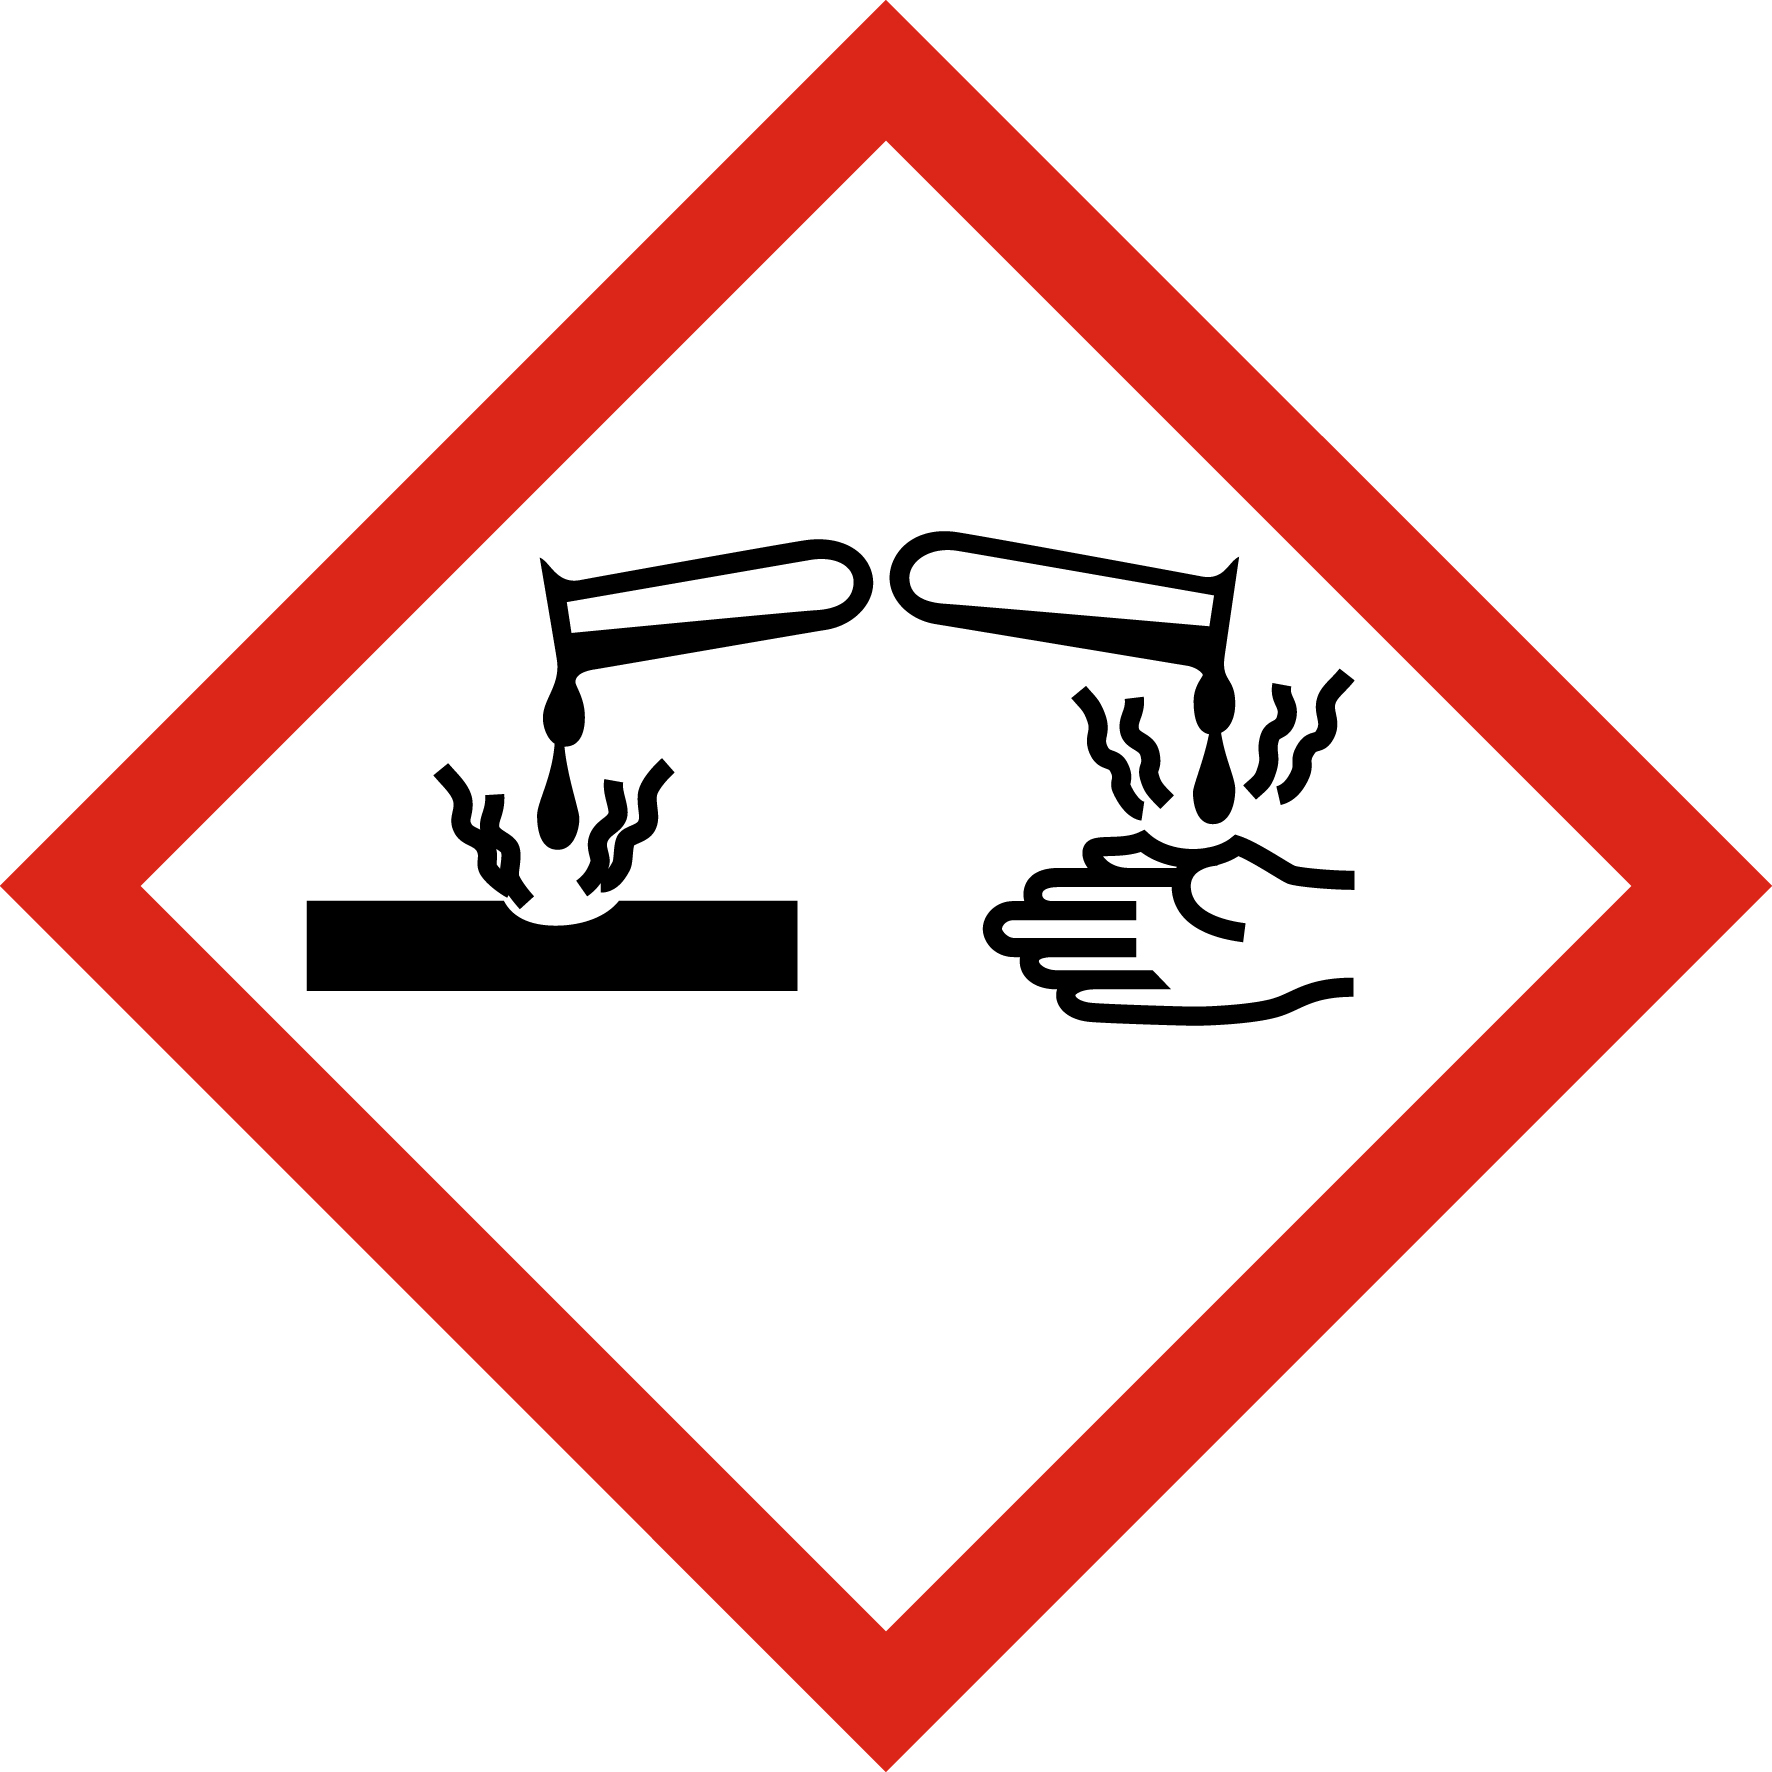
\includegraphics[scale=0.1]{Images/SGH05_Corrosion.jpg} \\
        \hline
    \end{tabular}
\end{doc}
\clearpage

%%%% documents
\begin{doc}{Applications de quelques ions}
\vspace{-0.8cm}
\begin{center}
    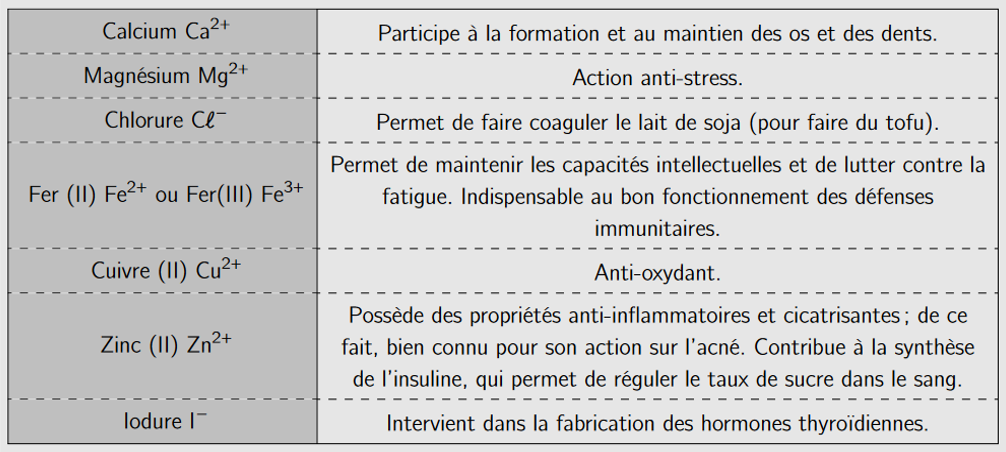
\includegraphics[scale=0.73]{Images/Ions.png}
\end{center}
\end{doc}

\begin{doc}{Identification de quelques ions}
\vspace{-0.8cm}
\begin{center}
    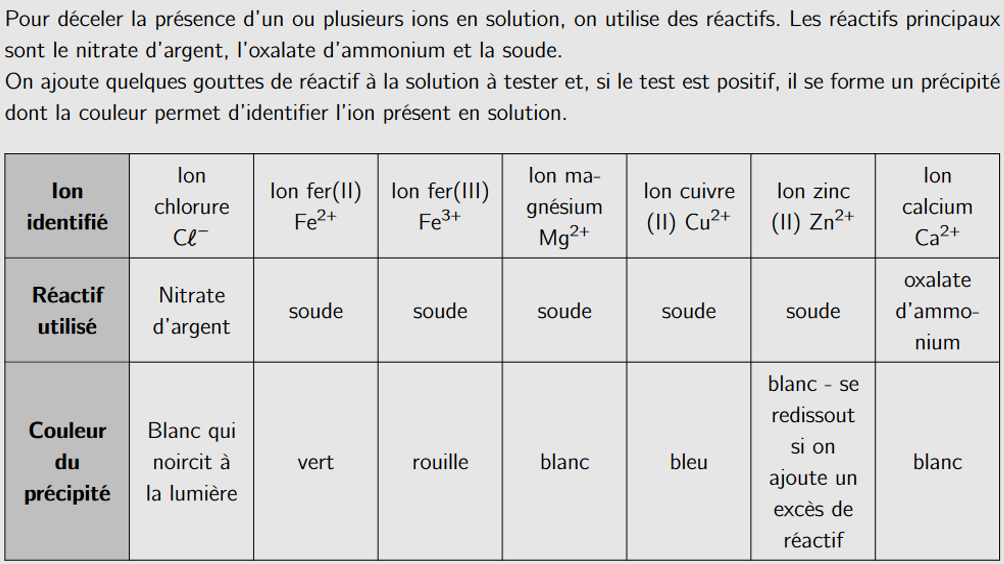
\includegraphics[scale=1]{Images/Ions_identification.png}
\end{center}
\end{doc}
\newpage
\begin{doc}{Définition et propriété d'un composé ionique}
\vspace{-0.5cm}
\begin{center}
    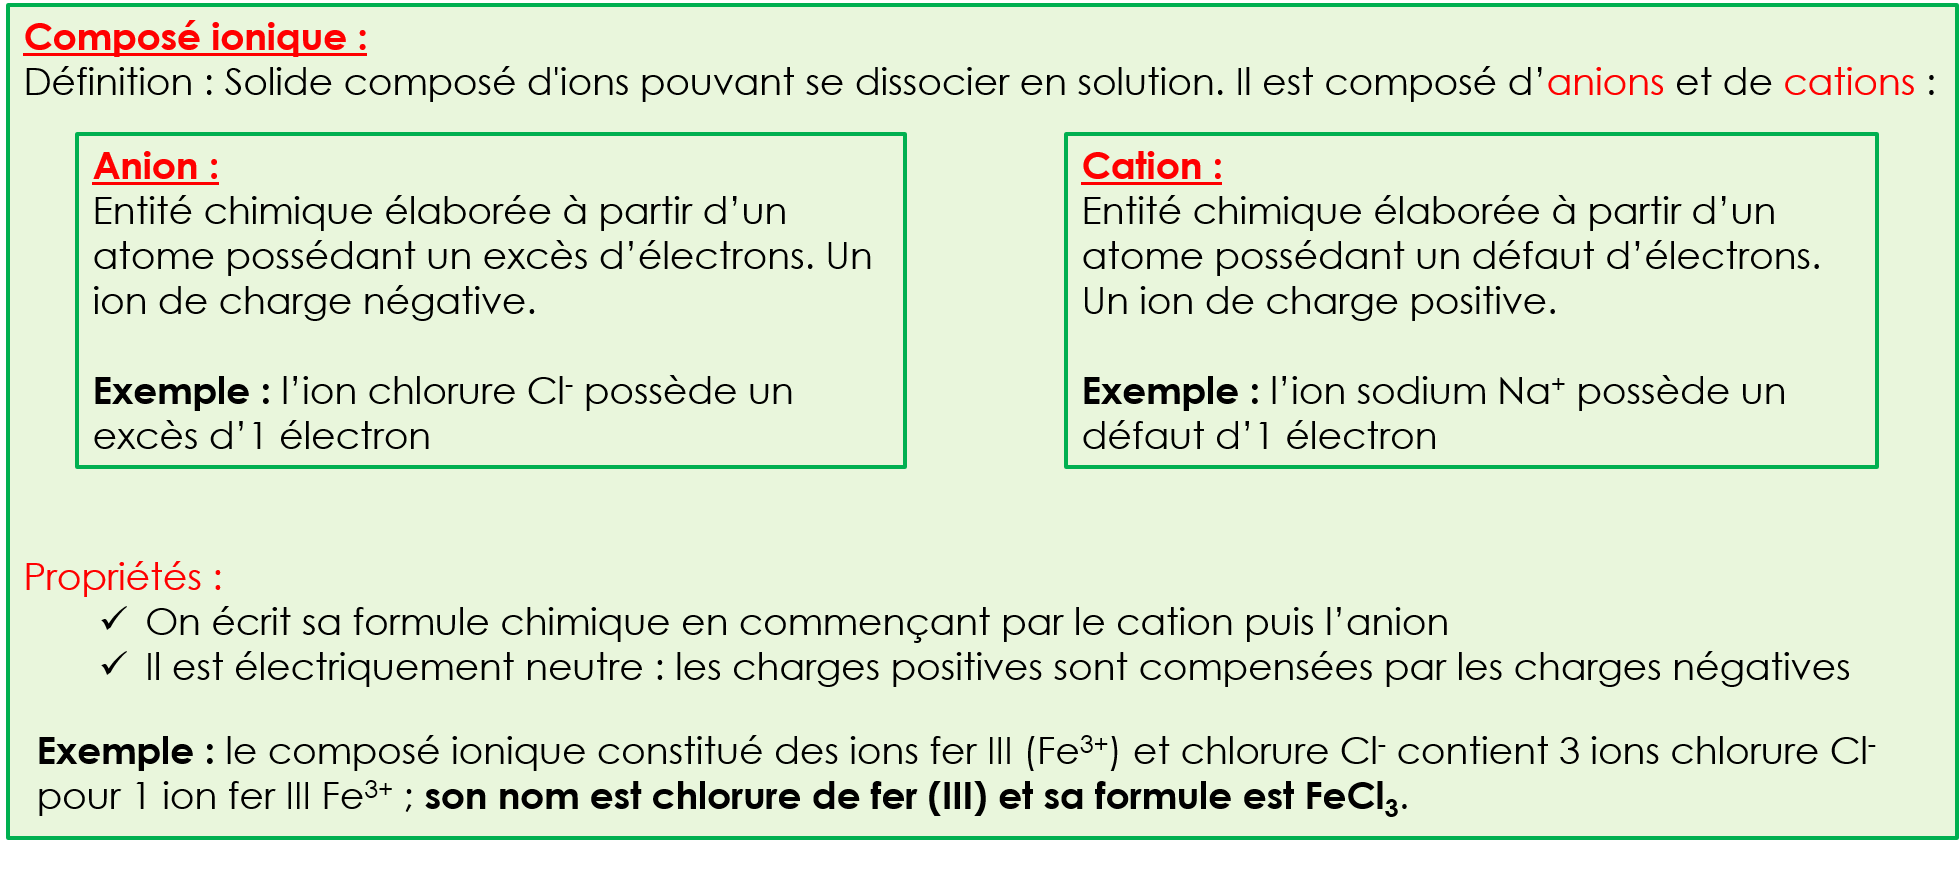
\includegraphics[scale=0.5]{Images/Solide_ionique.png}
\end{center}
\end{doc}

\begin{large}
    \textbf{\textcolor{red}{\underline{Travail à réaliser :}}}
\end{large}

\question{Rappeler la problématique.}{~}{0}
%\\
\question{Proposer un protocole expérimental permettant de vérifier les effets recherchés du nigari. Vous pourrez utiliser des schémas accompagnés de phrases explicatives.}{~}{0}

\begin{center}
\begin{mdframed}[style=titr, leftmargin=60pt, rightmargin=60pt, innertopmargin=7pt, innerbottommargin=7pt, innerrightmargin=8pt, innerleftmargin=8pt]

\begin{center}
\begin{Large}
    \textcolor{red}{Appeler le professeur pour vérifier votre protocole.}
\end{Large}
\end{center}
\end{mdframed}
\end{center}

%\\
\question{Mettre en œuvre le protocole expérimental précédent.}{}{0}
%\\
\question{Noter vos observations.}{~}{0}
%\\
\question{\textbf{\underline{Interprétation :}} en déduire les ions présents dans le nigari.}{~}{0}
%\\
\question{\textbf{\underline{Conclusion :}} à l'aide du document 3, en déduire le nom et la formule du composé ionique constituant le nigari. Indiquer les effets bénéfiques et applications du nigari.}{~}{0}
\newpage

\begin{difficile}{Bilan à retenir}
On distingue 3 types d'entités chimiques dans la matière à l'échelle microscopique : 
\begin{center}
    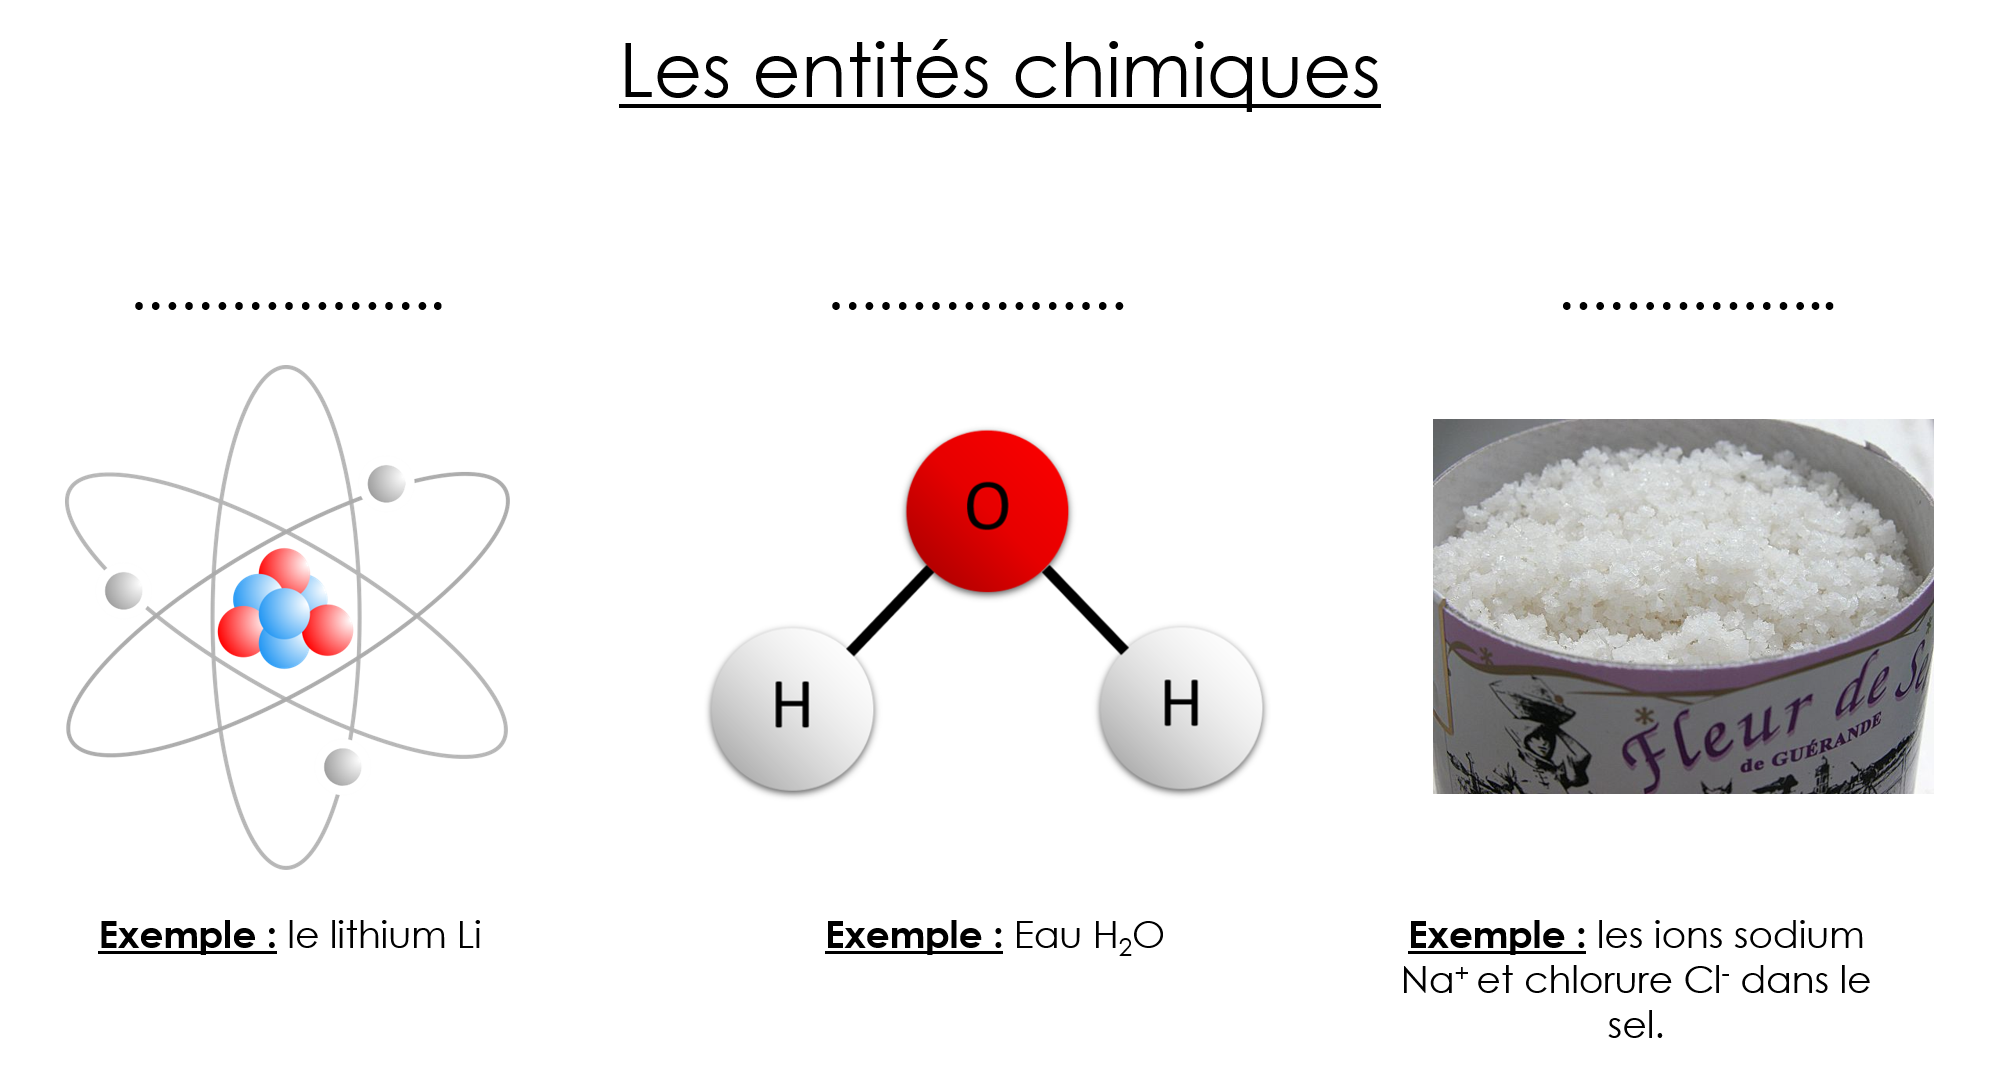
\includegraphics[scale=0.5]{Images/Entites_chimiques_acompleter.png}
\end{center}
La matière est globalement neutre à l'échelle macroscopique. Les espèces ioniques sont donc constituées d'au minimum deux types d'entités : des anions et des cations dans des proportions telles que \textbf{\underline{le solide ionique est globalement neutre électriquement}}.\\
\textcolor{red}{Notations} : 
\begin{itemize}
    \item Les ions en solutions aqueuses s'écrivent comme le symbole de l'atome auquel on met en exposant le nombre de charges de l'ion. \textbf{Exemple :} l'ion sodium s'écrit \chemform{Na^+} et l'ion chlorure s'écrit \chemform{Cl^-}.    
    \item La formule chimique d'un solide ionique s'écrit en commençant par le cation puis l'anion. 
    \textbf{Exemple :} le chlorure de sodium solide s'écrit \chemform{NaCl(s)} 
    \item On écrit en indice le nombre de chaque ion forment le composé ionique afin que la charge globale soit neutre. \textbf{Exemple :} \chemform{NaCl} est composé d'1 ion sodium \chemform{Na^+} et d'1 ion chlorure \chemform{Cl^-}
\end{itemize}
\end{difficile}

\begin{mdframed}[style=autreexo]
\textbf{\'{E}crire la formule chimique des solides ioniques à partir des ions suivants :}
\begin{itemize}[label=\textbullet, font=\large]
    \item l'ion argent \chemform{Ag^+} et l'ion nitrate \chemform{NO_3^{-}} forment le solide \gap{..............} 
    \item l'ion fluorine \chemform{F^-} et l'ion calcium \chemform{Ca^{2+}} forment le solide \gap{..............}
    \item l'ion hydroxyde \chemform{OH^-} et l'ion magnésium \chemform{Mg^{2+}} forment le solide \gap{..............}
    \item l'ion zinc \chemform{Zn^2+} et l'ion phosphate \chemform{PO_4^{3-}} forment le solide \gap{..............}
\end{itemize}
\end{mdframed}
%\newpage
%\papiermillimetre